\subsection{Block Design}

We are interested in the simple block experiment in this research, so we are 
first to the fit block design to ordinary least square regression in order to
define the basic relationship between neural signal and blood pressure. Here, 
we assume the error from data is followed independent and identically normal
distribution and constant variance.

\begin{figure}[!h]
\centering
\begin{subfigure}{.42\textwidth}
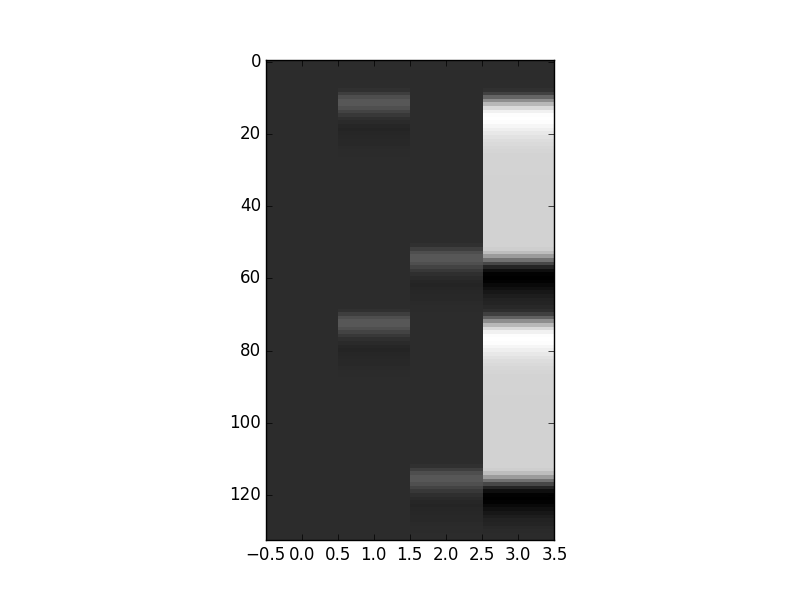
\includegraphics[scale=0.45]{block_design_mat}
\centering
\caption{Design Matrix for Block Design\label{fig:blockDM}}
\end{subfigure}%
\begin{subfigure}{.48\textwidth}
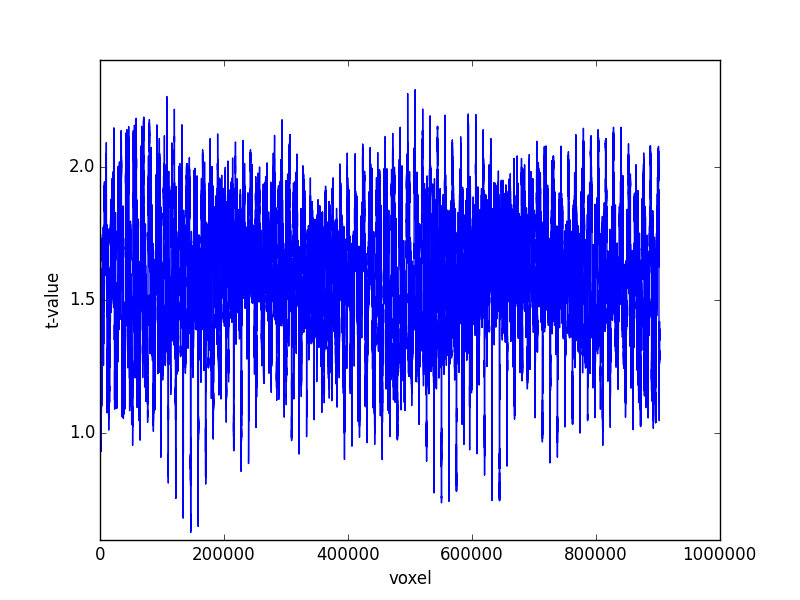
\includegraphics[scale=0.45]{task001_run001_T_value_block}
\centering
\caption{T-value of $\hat{\beta_{3}}$ in Block Design OLS\label{fig:tvalOLS}}
\end{subfigure}
\caption{Block Design Model\label{fig:blockDM}}
\end{figure}

Since the $\hat{\beta_{3}}$ in 2 demission is not easy to recognize which voxels
are significantly active, we would like to reshape to 3 demission as the brain 
shape. Then, we plot the $\hat{\beta_{3}}$ and P-value of front, middle and 
back perspectives respectively.

\begin{figure}[!h]
\centering
\begin{subfigure}{.45\textwidth}
  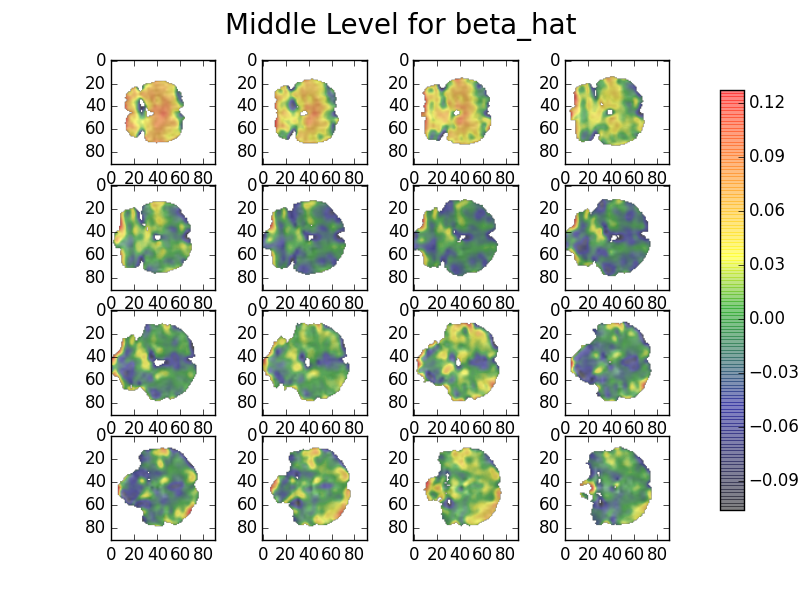
\includegraphics[scale=0.4]{block_beta_middle_map}
\end{subfigure}%
\begin{subfigure}{.5\textwidth}
  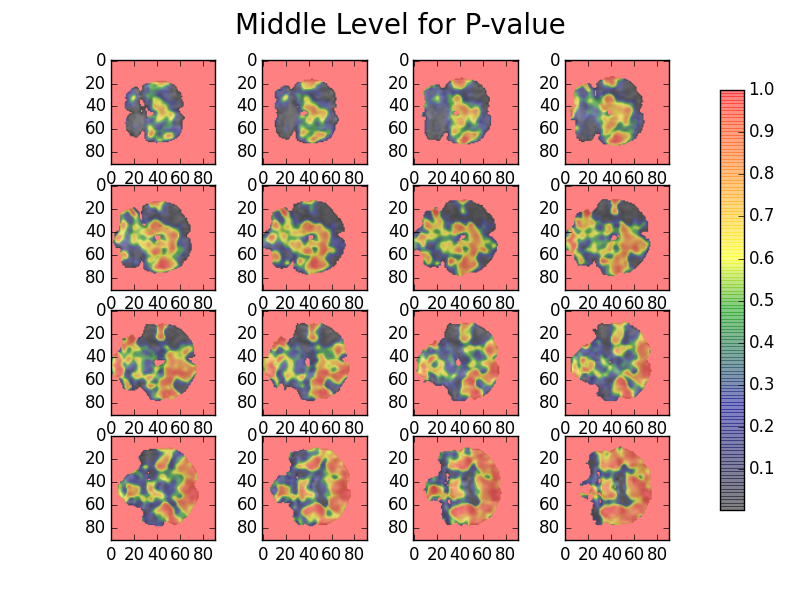
\includegraphics[scale=0.4]{block_p_middle_map}
  \centering
\end{subfigure}
\caption{Middle Perspective of Brain in Block Design\label{fig:mpBrain}}
\end{figure}

In the $\hat{\beta}$ map, the warmer color is showing $\hat{\beta}$ is 
bigger, which means there is higher positive relationship between neural signal and
blood pressure. However, if the color is more likely yellow, it means 
$\hat{\beta}$ is close to 0, so there is less or no relation at all. 
Therefore, We think the voxels are highly active during the experiment test 
located at the center of front and back brain. On the other hand, in the middle
brain, majority of voxel are showing the negative relationship between neural
signal and blood pressure.

In the p-value map, the dark region is showing higher confidence on the 
$\hat{\beta}$ value. the color of regions are more bright, we can judge that 
these voxels are not related to our experiment test. Therefore, We could not 
find many regions are highly significantly, however, if the voxels are on the 
edge of brain, most of them did not provide any information in the blood 
pressure, which makes sense to us.

\begin{figure}[!h]
\centering
\begin{subfigure}{.46\textwidth}
  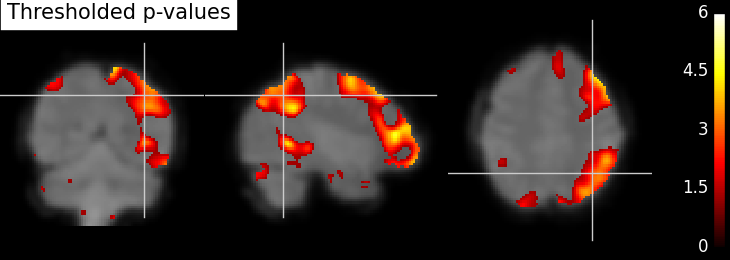
\includegraphics[scale=0.41]{block_p_map_0_05}
  \centering
\end{subfigure}%
\begin{subfigure}{.44\textwidth}
  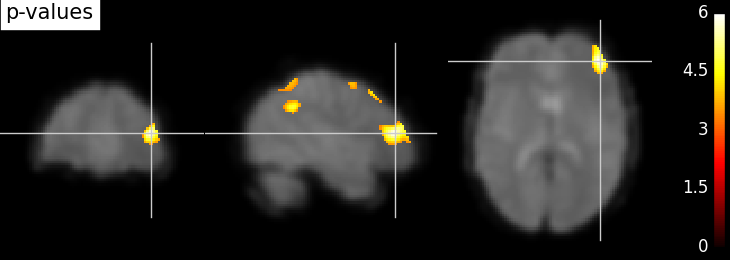
\includegraphics[scale=0.41]{block_p_map}
  \centering
\end{subfigure}
\caption{Highly Significant Voxels in the Block Design\label{fig:hsVoxels}}
\end{figure}

In the left image, we set the threshold to 0.05, so find the red region contains
highly significant active voxels. In the right image, as Bonferroni correction
theory, we decide to set the threshold to 0.05/133, then we get a few very 
significant regions. However, most of them are located at the edge of brain, 
which does not make sense in the common knowledge. Therefore, we did not firmly
believe this results, so in the next section, we are going to check heteroscedasticity
test.

\subsection{Heteroscedasticity Test}
In the paper, it introduces that there is non-constant variance of blood 
measurement in the dataset, which means it breaks the assumption of ordinary 
least squares. If the variance of the Y is not constant, then the error variance
will not be constant because it assumes there is linear relationship between 
true Y and X. The most common form of such heteroscedasticity in Y is that the 
variance of Y may increase as the mean of Y increases, for data with positive X
and Y. We would like to apply heteroscedasticity test, called white test in order to 
statistical test on variance.

\begin{enumerate}
\item Set the null hypothesis: no heteroscedasticity; Ha: there is heteroscedasticity
\item Estimate by OLS, save squared residuals in $e^2$
\item Regress $e^2$ on all variables, their squares and all possible non-redundant cross-products
\item Form the auxiliar regression: $n R^2 ~ X^2(p)$
\item Reject if $n R^2$ is too large
\end{enumerate}
Intuition: The auxiliar model can be seen as trying to model the variance of 
the error term. If the $R^2$ of this auxiliar regression were high, then we could
explain the behavior of the squared residuals, providing evidence that they are
not constant.

\begin{figure}[!h]
\centering
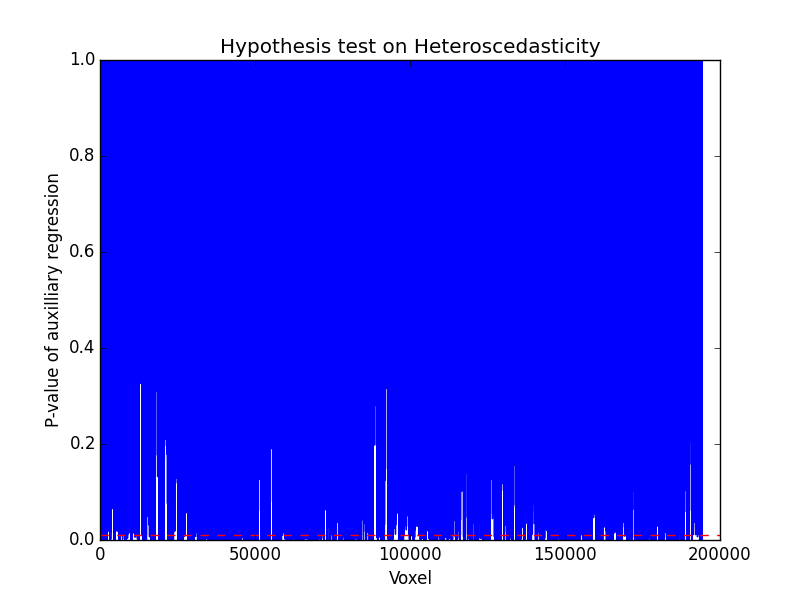
\includegraphics[scale=0.5]{block_p_auxi}
\caption{P value for Heteroscedasticity Test in Block Design}
\end{figure}

In the figure, we can see only few points under the red line, which voxels are
been rejected the null hypothesis test. 

The result I got is that there are total 194287 voxels, but only 3868 voxels 
have the significant P value which means reject our null hypothesis. Because 
only 2\% voxels have the constant variance, we judge the most voxels keep 
non-constant variance in the dataset. Therefore, we could not apply ordinary 
least squares regression, however, a weighted least squares linear regression 
may be the preferred method of dealing with non-constant variance of error.

